\section{Modelling the MW}
\begin{table}[H]\label{tab:models}
%\begin{center}
\begin{scriptsize}
\begin{tabular}{c c c c c }
\hline
Component  &  Besla07 &  LM2010 & Roeland12 & Vera-Helmi13 \\
\hline
Disk Model & Miyamoto-Nagai   & Miyamoto-Nagai &  & Miyamoto-Nagai \\
Disk Mass($M_{\odot}$) & $5.5^{10}$  & $1.0 \times 10^{11}$ & &  $1.0 \times 10^{11}$ \\
Disk Param & $R_d = 3.5$, $z=r_{disk}/5.0$  & $\alpha=1$, $a=6.5 kpc$, $b=0.6 kpc$ & &, $a=6.5kpc$, $b=0.26Kpc$\\
Bulge Model & Hernquist & Hernquist &  & Hernquist\\
Bulge Mass($M_{\odot}$) & $10^{10}$  &$3.4 \times 10^{10}$ & & $3.4\times 10^{11}$\\
Bulge Param & $0.6 kpc$ &  $c=0.7kpc$  & $0.6Kpc$ & $0.7 Kpc$\\
DM halo Model & NFW  & Triaxial \ref{sec:LM10}  & Hernquist(NFW) & Triaxial-Oblate\\
DM halo mass($M_{\odot}$) & $10^{12}$ &$ \times 1.5 \times 10^{12}$ & $10^12$ &\\
Solar Velocity &    &    & 239  & 225.2\\
Halo Param & $c=11, r_{vir} = 258Kpc$ & $r_{halo} = 12 Kpc$ & & $d=12kpc, q_z=0.9, q_1=1.38$\\
 & & & &  $q_2=1, q_3=1.36, \phi=97, r_a=30 kpc$ \\
Solar distance $R_{\odot}$ (kpc) & 8.0 & 8.0  & & 8.0\\
reference &\href{http://adsabs.harvard.edu/abs/2007ApJ...668..949B}{Besla07} & \href{http://bit.ly/1fXtla9}{LM2010} & & \href{http://adsabs.harvard.edu/abs/2013ApJ...773L...4V}{Vera13} \\
\hline
\end{tabular}
\end{scriptsize}
%\end{center}
\end{table}




\begin{figure}[H]\label{MWBesla07}
\centering
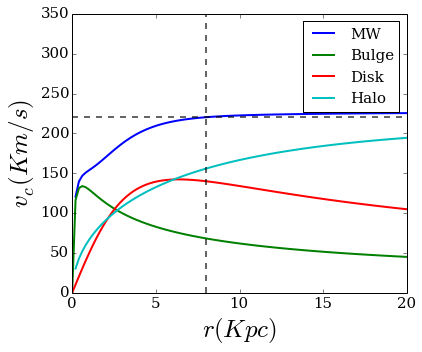
\includegraphics[scale=0.7]{../figures/MWBEsla07.png}
\end{figure}



\begin{figure}[H]\label{MWLM10}
\centering
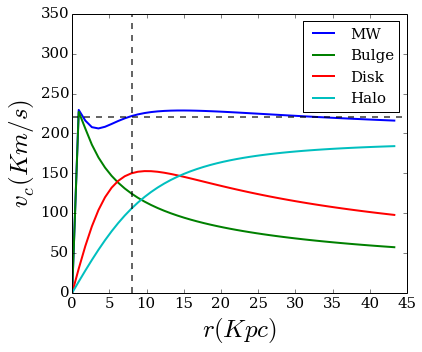
\includegraphics[scale=0.7]{../figures/MWLM10.png}
\end{figure}

\subsection{Vera-Ciro \& Helmi models}

\begin{equation}
\Phi_s(r) = v_{halo}^2 ln(\tilde{r}^2 + d^2)
\end{equation}

\begin{equation}
\tilde{r} = \dfrac{r_a + t_T}{r_a + r_A}r_A
\end{equation}

\begin{equation}
r_A^2 = x^2 + y^2 + \dfrac{z^2}{{q_z}^2} 
\end{equation}

\begin{equation}
r_T ^ 2 = C_1 x^2 + C_2 y^2 + C_3 xy + \dfrac{z^2}{q_3^2}
\end{equation}

Where $C_1, C_2, C_3$ are the same as in the triaxial model. 

Then the acceleration would be:

\begin{equation}
a = -\nabla \Phi 
\end{equation}

\begin{equation}
-\nabla \Phi = -v_{halo}^2 \dfrac{2 \tilde{r} }{ (\tilde{r}^2 + d^2)} \left(  \dfrac{d\tilde{r}}{dx} \hat{i} + \dfrac{d\tilde{r}}{dy} \hat{j} + \dfrac{d\tilde{r}}{dz} \hat{k}    \right)
\end{equation}

To evaluate this derivatives the following expressions are useful:

\begin{equation}
\dfrac{\partial r_T}{\partial x} = \dfrac{C_1x + C_3y/2}{(C_1X^2 + C_2y^2 + C_3xy + z^2/q_3^2)^{1/2}}
\end{equation}

\begin{equation}
\dfrac{\partial r_T}{\partial y} = \dfrac{C_2y + C_3x/2}{(C_1X^2 + C_2y^2 + C_3xy + z^2/q_3^2)^{1/2}}
\end{equation}

\begin{equation}
\dfrac{\partial r_T}{\partial z} = \dfrac{z/q_3^2}{(C_1X^2 + C_2y^2 + C_3xy + z^2/q_3^2)^{1/2}}
\end{equation}

\begin{equation}
\dfrac{\partial r_A}{\partial x} = \dfrac{x}{(x^2 + y^2 + z^2/{q_z}^2)^{1/2}}
\end{equation}

\begin{equation}
\dfrac{\partial r_A}{\partial y} = \dfrac{y}{(x^2 + y^2 + z^2/{q_z}^2)^{1/2}}
\end{equation}

\begin{equation}
\dfrac{\partial r_A}{\partial z} = \dfrac{z/q_z^2}{(x^2 + y^2 + z^2/{q_z}^2)^{1/2}}
\end{equation}

\begin{equation}
\dfrac{\partial \tilde{r}}{\partial \alpha} = \dfrac{\left( \dfrac{dr_T}{d\alpha} r_A + r_T \dfrac{dr_A}{d\alpha}\right) (r_a + r_A) - (r_a + r_T)r_A \dfrac{dr_A}{d\alpha} }{(r_a^2 + r_A^2)}
\end{equation}

Where $\alpha$ stands for the $x, y, z$

With these definitions the acceleration terms are:

\begin{equation}
a_x = - \dfrac{v_{halo}^2 2 \tilde{r}}{(\tilde{r}^2 + d^2)} \dfrac{\partial \tilde{r}}{\partial x}
\end{equation}

\begin{equation}
a_y = - \dfrac{v_{halo}^2 2 \tilde{r}}{(\tilde{r}^2 + d^2)} \dfrac{\partial \tilde{r}}{\partial y}
\end{equation}

\begin{equation}
a_z = - \dfrac{v_{halo}^2 2 \tilde{r}}{(\tilde{r}^2 + d^2)} \dfrac{\partial \tilde{r}}{\partial z}
\end{equation}


